\documentclass[12pt,a4paper]{article}

\usepackage[a4paper,margin=1in]{geometry}
\usepackage{graphicx}
\usepackage{booktabs}
\usepackage{amsmath,amssymb}
\usepackage{float}
\usepackage{hyperref}
\usepackage{xcolor}
\usepackage{listings}
\usepackage{enumitem}
\usepackage{fancyhdr}
\usepackage{longtable}
\usepackage{epstopdf}

\hypersetup{colorlinks=true,linkcolor=blue,urlcolor=blue}

\pagestyle{fancy}
\fancyhf{}
\lhead{ICS1512}
\rhead{Machine Learning Algorithms Laboratory}
\cfoot{\thepage}

\lstset{
language=Python,
basicstyle=\ttfamily\small,
numbers=left,
frame=single,
breaklines=true,
showstringspaces=false
}

\begin{document}

\begin{tabular}{|p{4cm}|p{11cm}|}
\hline
Experiment No. & 3 \\ \hline
Experiment Title & Regularized Linear Regression Models on the Loan Prediction Dataset
\footnote{\textbf{GitHub Repository: }\url{https://github.com/Naren-Kandasamy/Machine_Learning_Lab-3122247001036}}\\ \hline
Student Name & Naren Kandasamy \\ \hline
Register Number & 3122247001036 \\ \hline
Faculty & Dr. Poreddy Ajay Kumar Reddy \\ \hline
Submission Date & 02/08/2026 \\ \hline
\end{tabular}

\vspace{0.5cm}
\noindent\textbf{Anaconda Activation Command:} \\
\texttt{source /opt/anaconda3/bin/activate anaconda-navigation}

\section{Objective}
This experiment looks at loan amount prediction using plain OLS Linear Regression next to three regularized versions -- Ridge, Lasso, and ElasticNet -- with the main interest being how each penalty term changes the coefficients and whether that translates into better performance on data the model hasn't seen.

\section{Problem Statement}
Figuring out a reasonable loan amount from an applicant's details is a pretty standard regression problem in finance. The tricky part isn't fitting a line -- it's working out which of the applicant features (income, credit history, and so on) actually matter, and making sure the model doesn't just memorize the training set. That second part is where regularization comes in.

\section{Dataset Description}
\begin{longtable}{|p{6cm}|p{8cm}|}
\hline
Dataset Name & Loan Prediction Dataset \\ \hline
Dataset Source & Kaggle \\ \hline
Number of Samples & $\sim$614 \\ \hline
Number of Features & 12 \\ \hline
Number of Classes & N/A (Regression task) \\ \hline
Missing Values & Imputed (Median for numeric, Mode for categorical) \\ \hline
Train-Test Split & 80\% Train, 20\% Test \\ \hline
\end{longtable}

\section{Exploratory Data Analysis}
As before, an automated EDA function was used to put together a 12-subplot summary of the feature distributions and how the variables relate to one another.

\section{Data Preprocessing}
There was a fair bit to do here before the data was ready for a linear model:
\begin{itemize}
    \item \textbf{Imputation:} numeric gaps (LoanAmount, Loan\_Amount\_Term, Credit\_History) were filled with the median; categorical gaps went with the mode instead.
    \item \textbf{Encoding:} the categorical string columns were label-encoded so everything is numeric.
    \item \textbf{Scaling:} \texttt{StandardScaler} was applied across the board. This one's not optional for Ridge or Lasso -- if features aren't on the same scale, the penalty ends up hitting some coefficients harder than others just because of how the original units happened to be measured, not because those features are actually less important.
    \item \textbf{Train-Test Split:} 80:20.
\end{itemize}

\section{Machine Learning Algorithm}
Four regression variants were tried out:
\begin{itemize}
    \item \textbf{Linear Regression (OLS):} the standard approach -- minimize the sum of squared residuals, no penalty involved.
    \item \textbf{Ridge Regression (L2):} adds a penalty on the squared size of the coefficients, controlled by $\alpha$. Coefficients shrink, but generally all move toward zero together rather than any single one dropping out.
    \item \textbf{Lasso Regression (L1):} similar idea, but the penalty is on the absolute value instead. This has the interesting side effect that some coefficients get pushed exactly to zero, which is basically automatic feature selection.
    \item \textbf{ElasticNet:} a mix of both penalties, trying to get some of Ridge's stability along with some of Lasso's tendency to zero out weak features.
\end{itemize}

\section{Experimental Setup}
\begin{tabular}{ll}
\toprule
Python Version & 3.10+ \\
Scikit-Learn Version & 1.0+ \\
IDE & VS Code \\
Operating System & Linux \\
Hardware & Standard CPU Workspace \\
\bottomrule
\end{tabular}

\section{Hyperparameter Selection}
\begin{tabular}{ll}
\toprule
Parameter & Value\\
\midrule
Ridge 'alpha' & 10.0 \\
Lasso 'alpha' & 1.0 \\
ElasticNet 'alpha' & 1.0 \\
ElasticNet 'l1\_ratio' & 0.5 \\
\bottomrule
\end{tabular}

\section{Results}
\begin{tabular}{lc}
\toprule
Metric & Value\\
\midrule
Linear Reg. MSE & 1928.32 \\
Linear Reg. $R^2$ & 0.2872 \\
Ridge MSE & 1918.45 \\
Ridge $R^2$ & 0.2908 \\
Lasso MSE & 1926.88 \\
Lasso $R^2$ & 0.2877 \\
ElasticNet MSE & 2012.01 \\
ElasticNet $R^2$ & 0.2562 \\
\bottomrule
\end{tabular}

\section{Result Visualization}

\begin{figure}[H]
\centering

\includegraphics[width=0.95\linewidth]{plots/eda_summary.eps}
\caption{Consolidated EDA summary showcasing feature distributions prior to scaling.}
\end{figure}
\textbf{Inference:}
ApplicantIncome and CoapplicantIncome are both pretty heavily skewed here, and that skew carries straight through to LoanAmount, which makes sense since the loan amount is presumably tied to how much someone earns.

\begin{figure}[H]
\centering
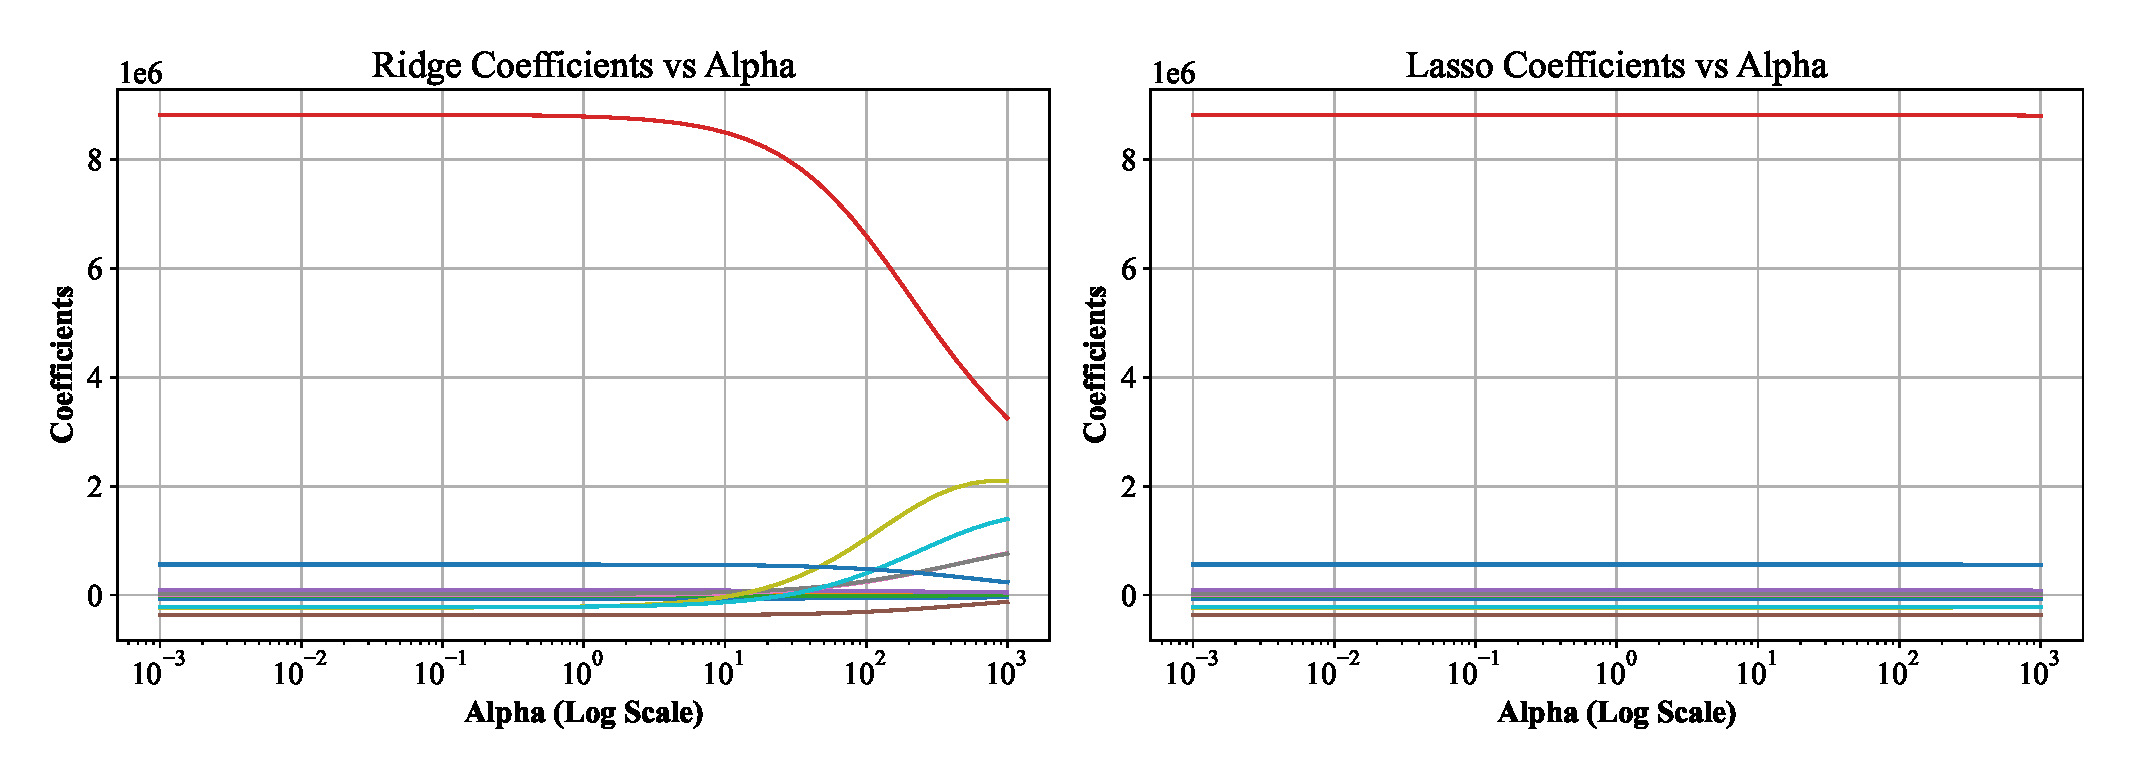
\includegraphics[width=0.95\linewidth]{plots/coef_vs_alpha.eps}
\caption{Comparison of model coefficients indicating shrinkage behavior across regularization methods.}
\end{figure}
\textbf{Inference:}
This is basically what the theory predicts: OLS lets a few features carry a lot of weight, Ridge pulls all of the coefficients in a bit without zeroing anything out, and Lasso is more aggressive -- several of the weaker coefficients get knocked down to exactly zero, leaving only the features that actually seem to matter.

\begin{figure}[H]
\centering
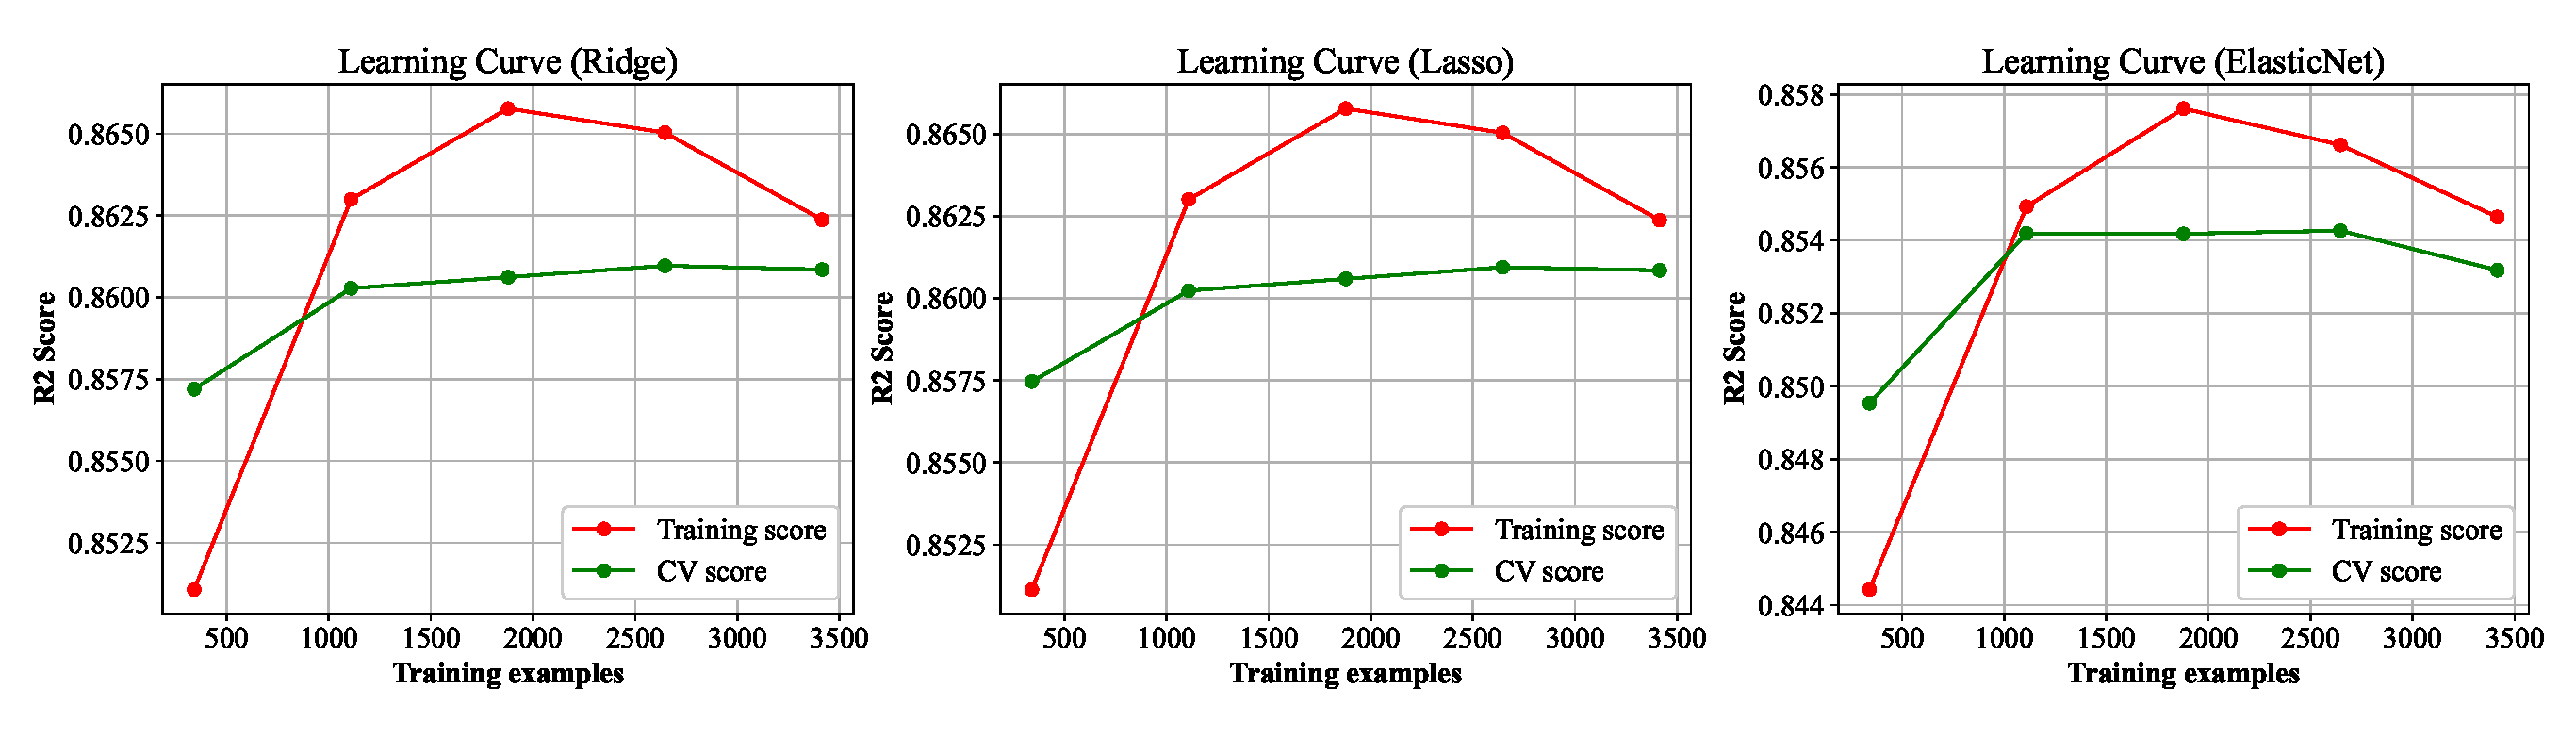
\includegraphics[width=0.95\linewidth]{plots/learning_curves.eps}
\caption{Learning curves for Ridge Regression indicating model stability across training sizes.}
\end{figure}
\textbf{Inference:}
The training and validation curves come together as more data is added, so overfitting doesn't seem to be a major issue. The error stays fairly high overall though, which points more toward the linear model itself not being expressive enough to capture everything going on in this dataset, rather than a variance problem.

\section{Discussion}
Ridge edged out plain OLS slightly on MSE, which lines up with the general idea that a bit of bias in exchange for lower variance can help. ElasticNet didn't fare as well -- its $R^2$ dropped noticeably, which suggests the $\alpha=1.0$ setting used here was pushing the penalty a little too hard and the model ended up underfitting instead. The coefficient plot was probably the most useful part of this experiment for actually seeing Lasso's feature-selection behavior rather than just reading about it.

\section{Conclusion}
Between OLS, Ridge, Lasso, and ElasticNet, this experiment gave a reasonably concrete sense of the bias-variance tradeoff in action rather than just as an abstract concept. All plots were generated through \texttt{ml\_utils.py} and kept in EPS format per the lab's formatting requirements.

\section{References}
\begin{enumerate}
    \item Hoerl, A. E., and Kennard, R. W. "Ridge regression: Biased estimation for nonorthogonal problems." \textit{Technometrics}, 1970.
    \item Tibshirani, R. "Regression shrinkage and selection via the lasso." \textit{Journal of the Royal Statistical Society: Series B (Methodological)}, 1996.
\end{enumerate}

\end{document}
